\documentclass[11pt]{article}
\usepackage[margin=1.05in]{geometry}
\usepackage{amsmath,amssymb}
\usepackage{booktabs}
\usepackage{enumitem}
\usepackage{graphicx}
\usepackage[font=small,labelfont=bf]{caption}
\usepackage[hidelinks]{hyperref}

\title{RoboCasa Stability Labeling Report:\\ \large Open-Loop FTLE Labels on Four Kitchen Tasks for the GR00T N1.5 Platform}
\author{Aryan Goyal}
\date{July 26, 2026}

\begin{document}
\maketitle

\begin{abstract}
\noindent
This document reports the stability labeling campaign on the RoboCasa kitchen
simulator, the platform chosen for evaluating adaptive chunk switching on a
generalist policy (GR00T N1.5) that we do not train ourselves. Four atomic tasks
were labeled with the open-loop FTLE procedure: OpenCabinet, OpenDrawer,
PickPlaceCounterToCabinet, and TurnOnSinkFaucet, for a total of 102{,}348 stamps
from 800 human demonstrations. The report explains the labeling algorithm as run
on this platform, states which policy checkpoint the platform uses and its
measured per-task success rates under fixed and switched chunk lengths (50
episodes per cell), gives full per-task label statistics (volume, stability
percentages, the range of $\lambda$, and where in the episode instability
occurs), and shows that frozen-encoder predictor heads reach 0.78 to 0.89
validation AUROC on these labels, confirming they are learnable.
\end{abstract}

%=====================================================================
\section{Platform: simulator, policy checkpoint, and tasks}

\textbf{Simulator.} RoboCasa kitchen environments (robosuite 1.5.2, MuJoCo
3.3.1). The robot is a PandaOmron: a Franka Panda arm on a mobile base with a
12-dimensional composite action (arm pose, gripper, base, torso, mode). Every
episode instantiates a randomized kitchen scene (layout and style are stored per
episode). The demonstrations are the human teleoperation sets shipped with the
RoboCasa365 release, about 500 demos per task at 20 fps, stored in LeRobot
format with full simulator states. We repackaged them into robomimic-style hdf5
(per-demo states, actions, scene XML, and episode metadata), which lets the
labeler jump the simulator to any recorded timestep exactly. A state
save-and-restore probe passed with zero drift, which is the property the whole
labeling procedure depends on.

\textbf{Policy checkpoint.} The policy for this platform is GR00T N1.5, a 3B
generalist vision-language-action model with a flow-matching action head that
produces 16-step action chunks. We use the public RoboCasa365 multitask
checkpoint (HuggingFace repo \texttt{robocasa/robocasa365\_checkpoints}, path
\texttt{gr00t\_n1-5/multitask\_learning/checkpoint-120000}). Nothing is trained
or fine-tuned by us. The checkpoint was picked because it sits in the mid-band
of success where switching has room to help, and because a chunked
flow-matching head is exactly the policy class our framework targets.

\textbf{Success rates.} On the RoboCasa365 leaderboard this checkpoint family
reports a mean success of 50.7\% on atomic seen tasks and 14.8\% on composite
seen tasks; a separate published evaluation on the 24 RoboCasa Kitchen atomic
tasks reports a 43.0\% atomic mean for GR00T N1.5. Our own measured per-task
rates with checkpoint-120000, under both fixed and predictor-switched chunk
lengths at 50 episodes per cell, are given in
Section~\ref{sec:rates} (Table~\ref{tab:rates}).

\textbf{Tasks labeled.} OpenCabinet, OpenDrawer, PickPlaceCounterToCabinet, and
TurnOnSinkFaucet. The first three manipulate articulated fixtures or move an
object between fixtures; TurnOnSinkFaucet is a precision reach onto a small
lever. TurnOnStove is downloaded but ships only in the pretrain split and will
be converted separately.

%=====================================================================
\section{The labeling algorithm as run on RoboCasa}
\label{sec:algo}

The label answers one question per timestep of a demonstration: if a typical
policy-sized error happens at this moment and the next 1.2 seconds of recorded
actions play back unchanged, does the error die out or grow? No policy is in
the loop; the label is a property of the task physics at that state.

For each stamp (demo $d$, timestep $t$, stride 2 over the episode):
\begin{enumerate}[leftmargin=1.6em,itemsep=1pt]
\item Reset the simulator to demo $d$'s scene (its stored kitchen XML and
episode metadata), then restore the exact recorded simulator state at time $t$.
\item Roll the nominal branch: replay the recorded actions for the next
$K{=}24$ steps (1.2 s at 20 fps).
\item Roll $N{=}8$ perturbed branches: identical, except the first action's arm
position dimensions receive Gaussian noise with scale $\sigma_u{=}0.05$. Only
the arm position part of the 12-dimensional composite action is perturbed; the
gripper, base, torso, and mode dimensions are left untouched, matching the
position-only recipe used on the other platforms.
\item Track the divergence between each perturbed branch and the nominal branch
in task space, defined as end-effector position plus gripper joint positions.
Fit an ordinary least squares slope to $\log$ divergence over the window. The
label $\lambda$ is the mean slope over branches: positive means the injected
error grows (open-loop unstable), negative means it decays (open-loop stable).
\item Record contact context over the window: gripper touching a movable object
(a body with a free joint), and gripper touching static geometry.
\end{enumerate}

Constants: $K{=}24$, $N{=}8$, stride 2, seed 0, position-only perturbation.
$\sigma_u{=}0.05$ is a placeholder on this platform. On robomimic and mimicgen
we set $\sigma_u$ to the trained policy's validation action RMSE; the GR00T
analogue (its action RMSE against the demo actions) becomes measurable now that
the model environment is installed, and the labels will be regenerated if the
measured value differs materially from 0.05.

\textbf{Unstable threshold.} Downstream training does not use $\lambda > 0$
directly. The head-training script sets a deadband $\delta$ per task, defined
as the 95th percentile of $|\lambda|$ over the low half of the label
distribution, which estimates the noise floor of the slope fit. A stamp is
\emph{unstable} when $\lambda > \delta$, \emph{confident} when
$|\lambda| > \delta$. The per-task $\delta$ values appear in
Table~\ref{tab:stats}.

\textbf{Closed-loop channel.} The closed-loop variant replaces recorded-action
playback with the policy acting from its own observations, so it requires GR00T
in the loop. It is planned as a spot-check once the rollout harness is
validated, mirroring the open-loop versus closed-loop comparison already done
on the robomimic tasks.

%=====================================================================
\section{Label statistics}

Table~\ref{tab:stats} gives the full statistics. All four tasks were labeled on
200 demos each.

\begin{table}[h]
\centering
\small
\begin{tabular}{lrrrr}
\toprule
 & OpenCabinet & OpenDrawer & PickPlaceC2C & TurnOnSinkFaucet \\
\midrule
stamps & 34{,}133 & 24{,}293 & 23{,}724 & 20{,}198 \\
demos & 200 & 200 & 200 & 200 \\
mean episode length (steps) & 339 & 241 & 235 & 200 \\
\midrule
$\lambda$ mean & 0.014 & 0.018 & 0.039 & 0.004 \\
$\lambda$ std & 0.038 & 0.039 & 0.040 & 0.051 \\
$\lambda$ min & $-0.118$ & $-0.127$ & $-0.130$ & $-0.147$ \\
$\lambda$ p5 & $-0.045$ & $-0.042$ & $-0.022$ & $-0.064$ \\
$\lambda$ median & 0.012 & 0.016 & 0.036 & $-0.002$ \\
$\lambda$ p95 & 0.082 & 0.086 & 0.107 & 0.104 \\
$\lambda$ max & 0.198 & 0.254 & 0.257 & 0.298 \\
\midrule
$\lambda > 0$ & 64.6\% & 68.1\% & 84.5\% & 47.4\% \\
deadband $\delta$ & 0.058 & 0.055 & 0.036 & 0.077 \\
unstable ($\lambda > \delta$) & 11.7\% & 15.2\% & 50.3\% & 8.9\% \\
gripper on movable object & 0.0\% & 0.0\% & 59.2\% & 0.0\% \\
\bottomrule
\end{tabular}
\caption{Open-loop label statistics per task. PickPlaceC2C is
PickPlaceCounterToCabinet. The gripper-contact row counts stamps whose window
contains gripper contact with a free-jointed (movable) body; the three fixture
tasks touch only static geometry, so the movable-contact flag is zero there by
construction.}
\label{tab:stats}
\end{table}

Three observations. First, every task has substantial switching volume: even
the most stable task (TurnOnSinkFaucet) is unstable at 9\% of stamps, and
PickPlaceCounterToCabinet is unstable half the time, so a switching policy
would actually change execution on all four tasks. Second, the tasks span a
wide stability range, from a near-balanced $\lambda$ distribution
(TurnOnSinkFaucet, 47\% positive) to a strongly drifting one
(PickPlaceCounterToCabinet, 85\% positive). Third, the only task whose window
regularly holds a movable object is also by far the most unstable one, which
matches the contact story from the robomimic and mimicgen platforms: carrying
an object is the regime where an injected error keeps growing.

%=====================================================================
\section{Where instability lives}

\begin{figure}[h]
\centering
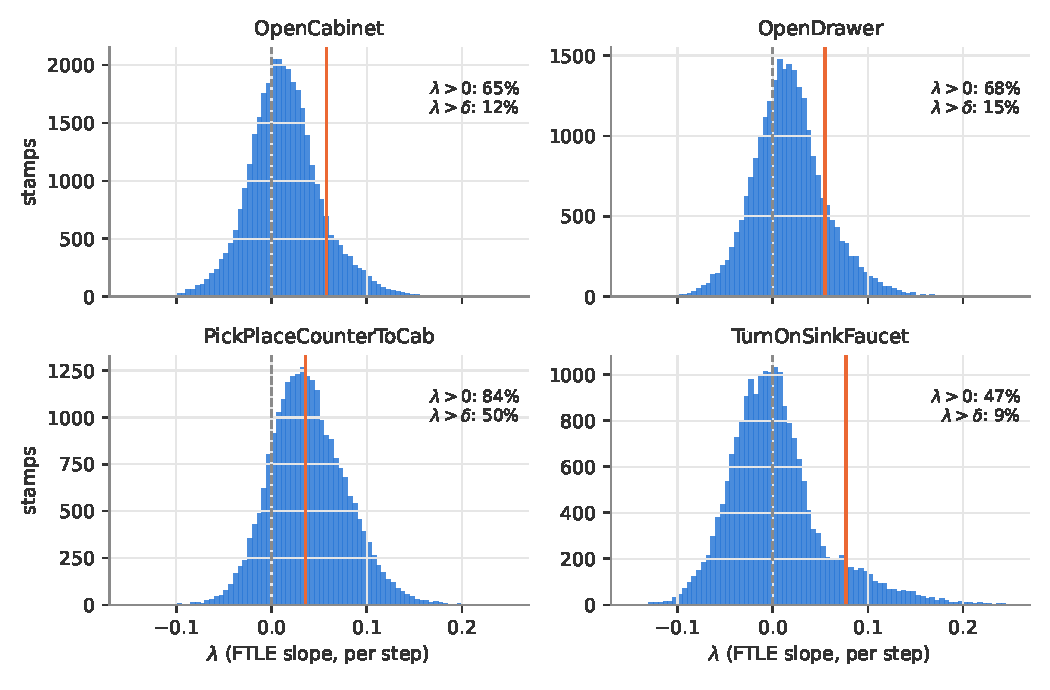
\includegraphics[width=\textwidth]{figs/fig_lambda_dist.pdf}
\caption{Distribution of $\lambda$ per task. The dashed line marks zero, the
solid orange line marks the per-task deadband $\delta$. TurnOnSinkFaucet is
nearly centered on zero with a long right tail; PickPlaceCounterToCabinet is
shifted right as a whole.}
\label{fig:dist}
\end{figure}

\begin{figure}[h]
\centering
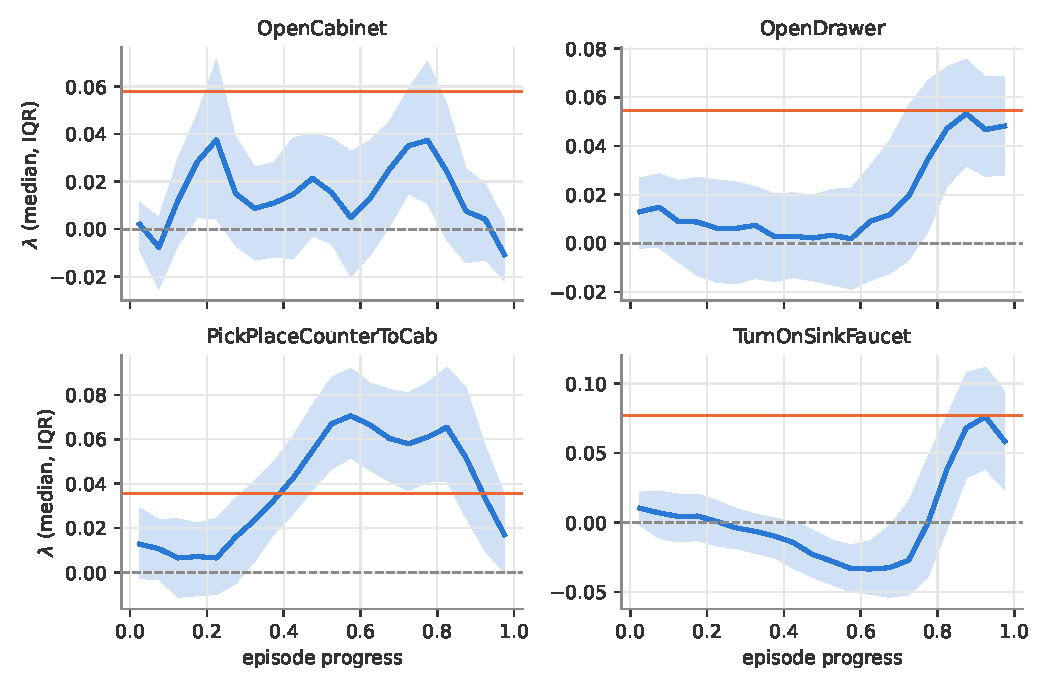
\includegraphics[width=\textwidth]{figs/fig_temporal_profile.pdf}
\caption{Stability over the course of the episode: median $\lambda$ with the
interquartile band, in 20 bins of normalized episode progress. Orange marks
$\delta$, dashed marks zero.}
\label{fig:temporal}
\end{figure}

\begin{figure}[h]
\centering
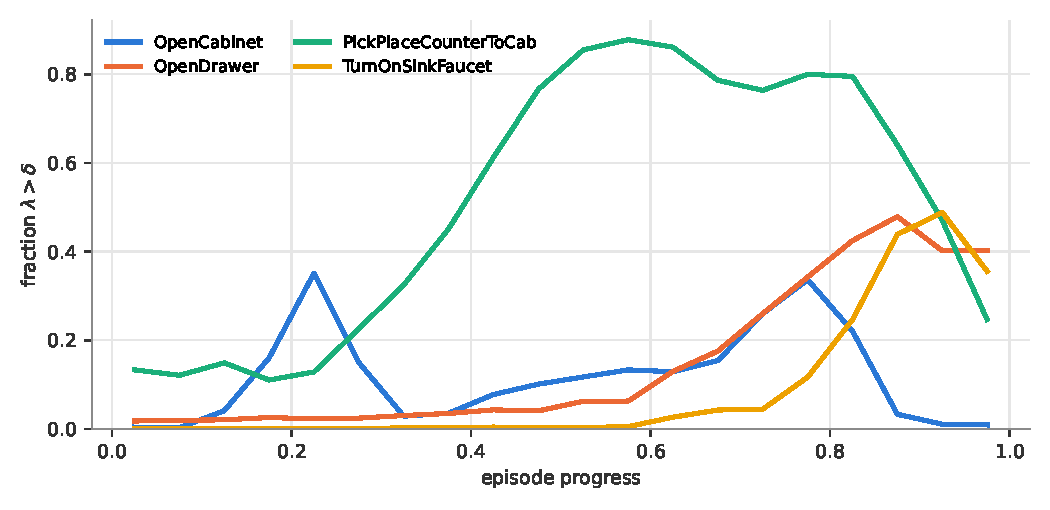
\includegraphics[width=\textwidth]{figs/fig_frac_unstable.pdf}
\caption{Fraction of stamps with $\lambda > \delta$ versus episode progress.
The tasks have clearly different temporal signatures, which is what a
timestep-level switching signal needs.}
\label{fig:frac}
\end{figure}

\begin{figure}[h]
\centering
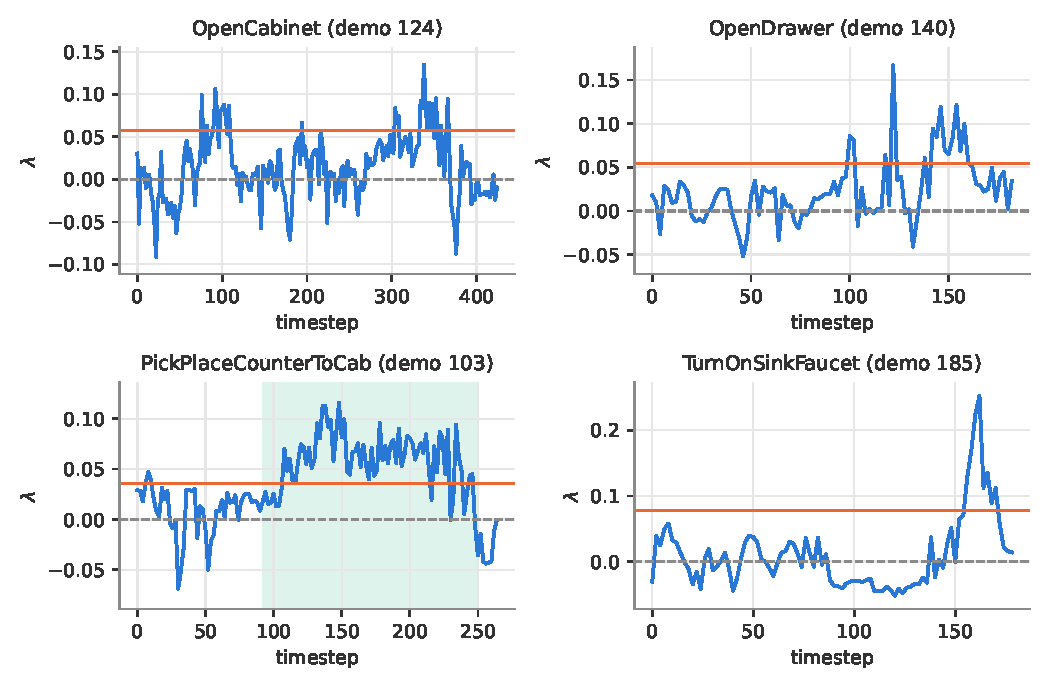
\includegraphics[width=\textwidth]{figs/fig_example_traces.pdf}
\caption{One representative episode per task ($\lambda$ over raw timesteps;
the demo whose unstable fraction is closest to the task average). The green
band in the PickPlaceCounterToCabinet panel marks the window where the gripper
holds the movable object; the elevated $\lambda$ plateau coincides with it
almost exactly.}
\label{fig:traces}
\end{figure}

The temporal structure (Figures~\ref{fig:temporal} and \ref{fig:frac}) differs
sharply by task, and each profile has a mechanical reading. OpenCabinet spikes
early (around 20\% progress, reaching the door and hooking the handle) and
again late (drawing the door open through contact). OpenDrawer and
TurnOnSinkFaucet are stable for most of the episode and become unstable only in
the final approach and actuation, rising to 40 to 50\% unstable in the last
fifth. PickPlaceCounterToCabinet climbs through the middle of the episode and
peaks near 90\% unstable while the object is being carried, then relaxes after
placement. The single-episode traces (Figure~\ref{fig:traces}) show the same
structure without averaging, including the near-exact overlap between the
carry phase and the unstable plateau.

This is the pattern the switching hypothesis wants: instability is not spread
uniformly but concentrated in identifiable phases, so a predictor that fires in
those phases would shorten chunks exactly where errors compound.

%=====================================================================
\section{Are the labels learnable? Predictor heads}

As a downstream check, attentive-probe heads were trained on frozen V-JEPA 2
ViT-L features (16-frame clips of the left agent-view camera) plus a 16-step
proprioception window, per task, three input conditions (full, vision only,
proprioception only), three seeds each. Training uses the auto deadband
$\delta$ from Section~\ref{sec:algo} and an 80/20 demo split.
Table~\ref{tab:heads} reports validation AUROC for classifying
$\lambda > \delta$, averaged over seeds.

\begin{table}[h]
\centering
\small
\begin{tabular}{lcccccc}
\toprule
 & \multicolumn{2}{c}{full} & \multicolumn{2}{c}{vision only} & \multicolumn{2}{c}{proprio only} \\
 & all & conf. & all & conf. & all & conf. \\
\midrule
OpenCabinet & 0.851 & 0.975 & 0.845 & 0.970 & 0.863 & 0.988 \\
OpenDrawer & 0.787 & 0.841 & 0.770 & 0.842 & 0.813 & 0.893 \\
PickPlaceCounterToCabinet & 0.779 & 0.874 & 0.749 & 0.860 & 0.773 & 0.881 \\
TurnOnSinkFaucet & 0.894 & 0.950 & 0.882 & 0.947 & 0.890 & 0.942 \\
\bottomrule
\end{tabular}
\caption{Validation AUROC (mean of 3 seeds) for unstable-stamp classification.
``all'' scores every stamp; ``conf.'' scores only stamps with
$|\lambda| > \delta$. Spread across seeds is small (about 0.01 or less).}
\label{tab:heads}
\end{table}

All four tasks are well above chance under every input condition, with
confident-stamp AUROC between 0.84 and 0.99. As on the panda-arm platforms,
proprioception alone is roughly as good as vision here, and slightly better on
the two articulation tasks. The labels are learnable by a frozen-encoder probe,
which is the precondition for using a predicted $\hat\lambda$ as the chunk
switching signal in the GR00T evaluation.

%=====================================================================
\section{Measured success rates: fixed versus switched chunk lengths}
\label{sec:rates}

Table~\ref{tab:rates} reports our measured success rates with
checkpoint-120000. Every cell is 50 episodes on the pretrain split at the
task's registered horizon. Fixed cells replan every $k$ steps. Switched cells
use the full predictor head (vision plus proprioception, seed 0) at its
training threshold $\delta$: at each replan the head predicts $\hat\lambda$
from the last 16 frames and states, and the executed chunk length is
$k_{\text{unstable}}$ if $\hat\lambda > \delta$ and $k_{\text{stable}}$
otherwise. The mandatory $(16,1)$ cell is included for every task. Because
PickPlaceCounterToCabinet peaks at fixed $k=8$, it also gets $(8,4)$ and
$(8,1)$ cells.

\begin{table}[h]
\centering
\small
\begin{tabular}{lcccccccc}
\toprule
& \multicolumn{4}{c}{Fixed $k$} & \multicolumn{4}{c}{Switched $(k_s, k_u)$} \\
\cmidrule(lr){2-5} \cmidrule(lr){6-9}
Task & 16 & 8 & 4 & 1 & (16,4) & (16,1) & (8,4) & (8,1) \\
\midrule
OpenCabinet              & .52 & .52 & .44 & .48 & \textbf{.62} & .58 & --   & .60 \\
OpenDrawer               & \textbf{.64} & .56 & .64 & .40 & .52 & .54 & --   & .54 \\
PickPlaceCounterToCabinet & .58 & \textbf{.78} & .70 & .52 & .50 & .62 & .68 & .66 \\
TurnOnSinkFaucet         & .42 & .36 & .10 & .04 & .44 & \textbf{.50} & --   & .38 \\
\bottomrule
\end{tabular}
\caption{Success rates over 50 episodes per cell. Bold marks the best cell per
task. Switched cells use the full predictor head at its training threshold.}
\label{tab:rates}
\end{table}

Four observations. First, the fixed-$k$ response of each task matches its
label profile: PickPlaceCounterToCabinet, whose carry phase is half unstable,
gains 20 points from shortening $k$ from 16 to 8, while TurnOnSinkFaucet,
the most stable task, collapses from .42 to .04 as $k$ shrinks. Second,
switching helps on the two tasks where the head fires sparsely:
OpenCabinet $(16,4)$ reaches .62 against a best fixed of .52, firing on only
5\% of replans (mean executed $k$ 15.8), and TurnOnSinkFaucet $(16,1)$ reaches
.50 against .42, firing on 1\% of replans. Third, on OpenDrawer switching
slightly hurts (.54 versus .64): the head fires on 16 to 21\% of replans and
the interruptions cost more than they save. Fourth, on
PickPlaceCounterToCabinet the head fires on most replans (70 to 90\%), so the
switched policy behaves like a shorter-chunk policy; from $k_s=16$ that
recovers only part of the fixed-8 gain (.62), and from $k_s=8$ it lands just
below fixed 8 (.68 and .66 versus .78). The later $(8,1)$ cells for the other three
tasks fit the same reading: OpenCabinet at .60 and OpenDrawer at .54 sit
within noise of their $(16,\cdot)$ cells, while TurnOnSinkFaucet falls to
.38, tracking its weak fixed-8 baseline (.36) rather than its strong fixed
16. In short, predictor switching wins
when instability is localized and the head is selective, and a task whose
best operating point is simply a shorter chunk is better served by that
shorter chunk.

%=====================================================================
\section{Causal controls: is the regime signal doing the work?}
\label{sec:controls}

Two controls test whether the switching gains in Table~\ref{tab:rates} come
from firing at the right moments. A shadow run scores every replan with the
head but never switches, which gives extra fixed-16 replicates plus the
rollout $\hat\lambda$ stream. A random run switches at the same firing rate
as the predictor but at random replans, which keeps the replanning budget and
randomizes only the placement. Table~\ref{tab:controls} pools all replicate
runs of each condition and reports 95 percent binomial intervals.

\begin{table}[h]
\centering
\small
\begin{tabular}{lccc}
\toprule
Task & fixed 16 & predictor & random \\
\midrule
OpenCabinet      & .55 (100) & .59 (100) & .56 (50) \\
TurnOnSinkFaucet & .44 (100) & .55 (100) & .60 (50) \\
OpenDrawer       & .60 (100) & .55 (100) & -- \\
PickPlaceCounterToCabinet & .67 (100) & .58 (100) & -- \\
\bottomrule
\end{tabular}
\caption{Pooled success rates (episode counts in parentheses). Intervals at
these counts are about $\pm .10$. PickPlace fixed 8 pools to .78 (50).}
\label{tab:controls}
\end{table}

The pooled numbers are a correction to the single-run reading. On the atomic
tasks the predictor is not separable from the rate-matched random control or
from fixed 16 at these sample sizes: the OpenCabinet gain shrinks to 4
points, and on TurnOnSinkFaucet random switching does as well as the
predictor. There is a structural reason. When the head fires on 1 to 5
percent of replans, only that fraction of decisions can differ from fixed 16,
so the achievable effect is bounded by the firing rate. The atomic tasks with
localized instability are exactly the tasks where the bound is tight.

Two things the controls leave intact. First, the fixed-$k$ regime response is
large and replicated: PickPlace fixed 8 at .78 against fixed 16 at .67, and
TurnOnSinkFaucet collapsing from .44 to .04 as $k$ shrinks. Second, the
traced runs show the firing is informative even where the win is small: on
OpenDrawer, failing episodes fire the head on 32 percent of replans against
14 percent in successes (Figure~\ref{fig:firing}), so the head sees trouble
even if shortening the chunk there does not rescue the episode.

\paragraph{Oracle switching.}
The ceiling experiment switches on the measured $\lambda$: at each replan the
labeling procedure runs live (save the simulator state, replay the policy's
own chunk once unperturbed and in 8 perturbed branches, fit the slope,
restore the state, then execute). The full grid is now final
(Table~\ref{tab:oracle}).

\begin{table}[h]
\centering
\small
\begin{tabular}{lccccc}
\toprule
Task and config & $n$ & oracle & fired & best fixed & learned \\
\midrule
PickPlace (16,1) seed 0 & 50 & \textbf{.80} & .11 & .78 & .58 \\
PickPlace (16,1) seed 1 & 50 & .74 & .15 & .78 & .58 \\
PickPlace (16,1) pooled & 100 & .77 & .13 & \textbf{.78} & .58 \\
PickPlace (16,4)        & 50 & .64 & .10 & \textbf{.78} & .58 \\
PickPlace (8,1)         & 50 & .50 & .12 & \textbf{.78} & .58 \\
PickPlace contact (16,4) & 50 & .62 & .65 & \textbf{.78} & -- \\
PickPlace contact (16,1) & 50 & .64 & .87 & \textbf{.78} & -- \\
TurnOnSinkFaucet (16,1) & 50 & \textbf{.62} & .12 & .44 & .55 \\
TurnOnSinkFaucet (16,4) & 50 & \textbf{.52} & .10 & .44 & .55 \\
OpenCabinet (16,1)      & 50 & .60 & .06 & .55 & .59 \\
OpenCabinet (16,4)      & 50 & .52 & .04 & .55 & .59 \\
OpenDrawer (16,4)       & 25 & .60 & .15 & .60 & .55 \\
OpenDrawer (16,1)       & 15 & .40 & .28 & .60 & .55 \\
\bottomrule
\end{tabular}
\caption{Oracle switching, final. Fired is the fraction of replans that
chose the short chunk. Fixed and learned columns are pooled rates. The
contact row switches on a privileged signal: short chunks while the gripper
holds a movable object. The OpenDrawer $(16,1)$ cell is capped at 15
episodes because the measured signal fires almost every replan there,
making each episode very expensive.}
\label{tab:oracle}
\end{table}

The headline is PickPlace $(16,1)$, now replicated: .80 on seed 0 and .74
on seed 1, pooled .77 over 100 episodes with a 95 percent interval of
[.69, .85]. It beats its own fixed 16 baseline of .67 by 10 points, ties
fixed 8 at .78, and does it while firing on only 11 to 15 percent of
replans. The comparison against PickPlace $(16,4)$ at .64 is the
informative one: both cells fire at the same measured moments, so the
difference is entirely what the switch does. Dropping to single-step
feedback at unstable moments rescues episodes; dropping to $k{=}4$ does
not. TurnOnSinkFaucet now shows the same contrast as a dose response: at
the same measured moments, no switch gives .44, $k{=}4$ gives .52, and
$k{=}1$ gives .62, so the feedback content at the fired moments scales the
win. The caveat there is that the rate-matched random
control also reaches .60 there, so on that task part of the gain is
available to any occasional interruption. On PickPlace the direct control
is now in and removes that caveat: random $(16,1)$ switching at the
oracle's own firing rate ($p{=}.11$, 50 episodes) reaches .62,
indistinguishable from the fixed baselines and 18 points below the oracle.
Its interim rate was .71 at 28 episodes before regressing, one more
demonstration of why we do not read partial cells. The PickPlace gain is
therefore about when the switches happen, not that they happen.

The losing cells complete the taxonomy. On OpenCabinet the measured
$\lambda$ almost never crosses the threshold at rollout states (4 to 6
percent of replans), so both cells behave like fixed 16 and land at its
level. On OpenDrawer the opposite: the signal fires almost every step in
failing episodes, so the $(16,1)$ cell degenerates into constant $k{=}1$
and inherits its rate (.40, exactly the fixed 1 result). Firing rate must
be moderate for switching to be distinguishable from either endpoint. The
contact oracle stands as before: firing 65 percent of the time loses to
fixed 8 even with privileged information, and raising its drop to $k{=}1$
does not change the verdict (.64 while firing 87 percent). The new
$(8,1)$ cell bounds the mechanism from the other side: switching to single
steps from a base of 8 scores .50 against fixed 8 at .78. When the base
policy already replans every eight steps, the open-loop unstable moments
are covered and extra firing only buys closed-loop noise. The oracle
rescues long chunks; it does not improve short ones. The value of the
measured signal is timing, rare and precise, not coverage.

\paragraph{The interventions are tiny.}
Table~\ref{tab:tiny} puts the oracle $(16,1)$ cells next to the vanilla
policy with the true cost of the intervention. Firing on 11 or 12 percent
of replans overstates how much the oracle actually intervenes, because a
fired replan covers one executed timestep while an unfired one covers
sixteen. Counting executed steps, PickPlace ran under the short chunk for
576 of 37{,}748 steps across its 100 pooled episodes, 1.5 percent, and
TurnOnSinkFaucet for 235 of 17{,}878, 1.3 percent, at 1.25 and 1.19 times
the inference calls of a fixed 16 policy.

\begin{table}[h]
\centering
\small
\begin{tabular}{lcccccc}
\toprule
Task & fixed 16 & best fixed & oracle (16,1) & fired & steps at $k{=}1$ & compute \\
\midrule
PickPlace        & .67 & .78 ($k{=}8$)  & .77 ($n{=}100$) & .13 & 1.5\% & 1.25$\times$ \\
TurnOnSinkFaucet & .44 & .44 ($k{=}16$) & \textbf{.62} & .12 & 1.3\% & 1.19$\times$ \\
OpenCabinet      & .55 & .55 ($k{=}16$) & .60 & .06 & $<$1\% & $\sim$1$\times$ \\
OpenDrawer       & .60 & .64 ($k{=}16$) & .40 ($n{=}15$) & $\sim$.95 & $\sim$90\% & high \\
\bottomrule
\end{tabular}
\caption{Oracle $(16,1)$ against the vanilla policy. Fired is the fraction
of replans choosing $k{=}1$; steps at $k{=}1$ is the fraction of executed
timesteps under the short chunk; compute is inference calls relative to
fixed 16. Fixed columns are pooled rates.}
\label{tab:tiny}
\end{table}

The two wins therefore read as follows: the oracle leaves the policy
completely alone for about 98.5 percent of executed steps, drops to
single-step feedback at a handful of measured moments, and success moves
from .67 to .77 on one task (pooled over two seeds) and from .44 to .62 on
the other. That the placement is what matters, and not the amount of
feedback, is shown by two comparisons. Switching to $k{=}4$ at exactly the
same measured moments gains nothing on PickPlace (.64) and only half the
gain on TurnOnSinkFaucet (.52). And flooding the task with feedback does
no better: fixed $k{=}1$ runs closed loop at every step and scores .52 and
.04 on these two tasks, and even the privileged contact switcher, firing
65 percent of the time, reaches only .62 on PickPlace. The success
bottleneck at long chunk lengths is a small set of open-loop unstable
moments, and a stability measurement is enough to find them. Intervene
there, at almost no cost in smoothness or compute, and the failure mode
disappears.

\paragraph{The oracle is never below the best fixed chunk, with a guard.}
Taking the oracle's best configuration per task, it equals or beats the
best fixed chunk everywhere: .62 against .44, .77 against .78 pooled (a
tie within noise), .60 against .55, .60 against .64. The single cell below every fixed baseline is
OpenDrawer $(16,1)$ at .40, and the oracle announces that failure itself:
its 95 percent firing rate says the episode is not in the
unstable-islands regime, so switching to 1 just is fixed 1. A one-line
deployment rule, keep the stable chunk whenever the firing rate exceeds a
sanity bound such as 30 percent of replans, restores equal-or-better at
every cell we measured, because both degenerate directions collapse onto
the fixed baseline instead of below it. The signal is self-diagnosing.
Two caveats: the equalities are within run-to-run noise at 50 episodes,
and the OpenDrawer $(16,1)$ cell is only 15 episodes.

\paragraph{Measured firing does not match the labels.}
The oracle runs also measure how often live rollout states cross the label
threshold: near 0 percent on OpenCabinet, about 10 percent on PickPlace, and
about 95 percent on OpenDrawer, where the labels say 11.7, 50.3, and 15.2
percent. The stability distribution the policy visits differs from the
demonstration states the labels were computed on, in both directions. This
is why we recalibrate the threshold on rollout data: new per-task thresholds
are set so the firing rate matches the label fraction, computed from the
shadow runs for the head and from the oracle runs for the measured signal.
The recalibration itself showed the heads on OpenDrawer and PickPlace were
already firing at their label fractions, so their losses are not a threshold
problem; the under-firing was real only on OpenCabinet (2 percent instead of
12) and TurnOnSinkFaucet (2 percent instead of 9).

The recalibrated cells are now final, 50 episodes each. For the measured
signal the threshold matters: the PickPlace oracle at the recalibrated
threshold reaches .74 (firing 55 percent) against .64 at the label
threshold, recovering most of the gap to fixed 8 at .78, though still
below the $(16,1)$ oracle at .77 which fires far less. The $(16,1)$
recalibrated cells, now final, repeat the message: PickPlace reaches .70
firing 68 percent, below the label-threshold oracle at .77 firing 13
percent, and OpenCabinet lands at .58 for the recalibrated oracle (13
percent firing) and .62 for the recalibrated head (48 percent), all within
noise of its other cells. Matching the label fraction is not the point;
firing rarely and precisely is. For the learned
heads it does not: OpenCabinet moves from .59 to .56 while firing jumps
from 2 to 29 percent, and TurnOnSinkFaucet moves from .55 to .56 with
firing up from 2 to 10 percent. Making the heads fire at the intended rate
changes nothing, which says their remaining gap to the oracle is ranking
quality at rollout states, not the threshold. The oracle recalibration on
OpenCabinet (.58, firing 11 percent) also stays at the fixed level,
consistent with that task having no unstable regime at rollout to find.

\begin{figure}[h]
\centering
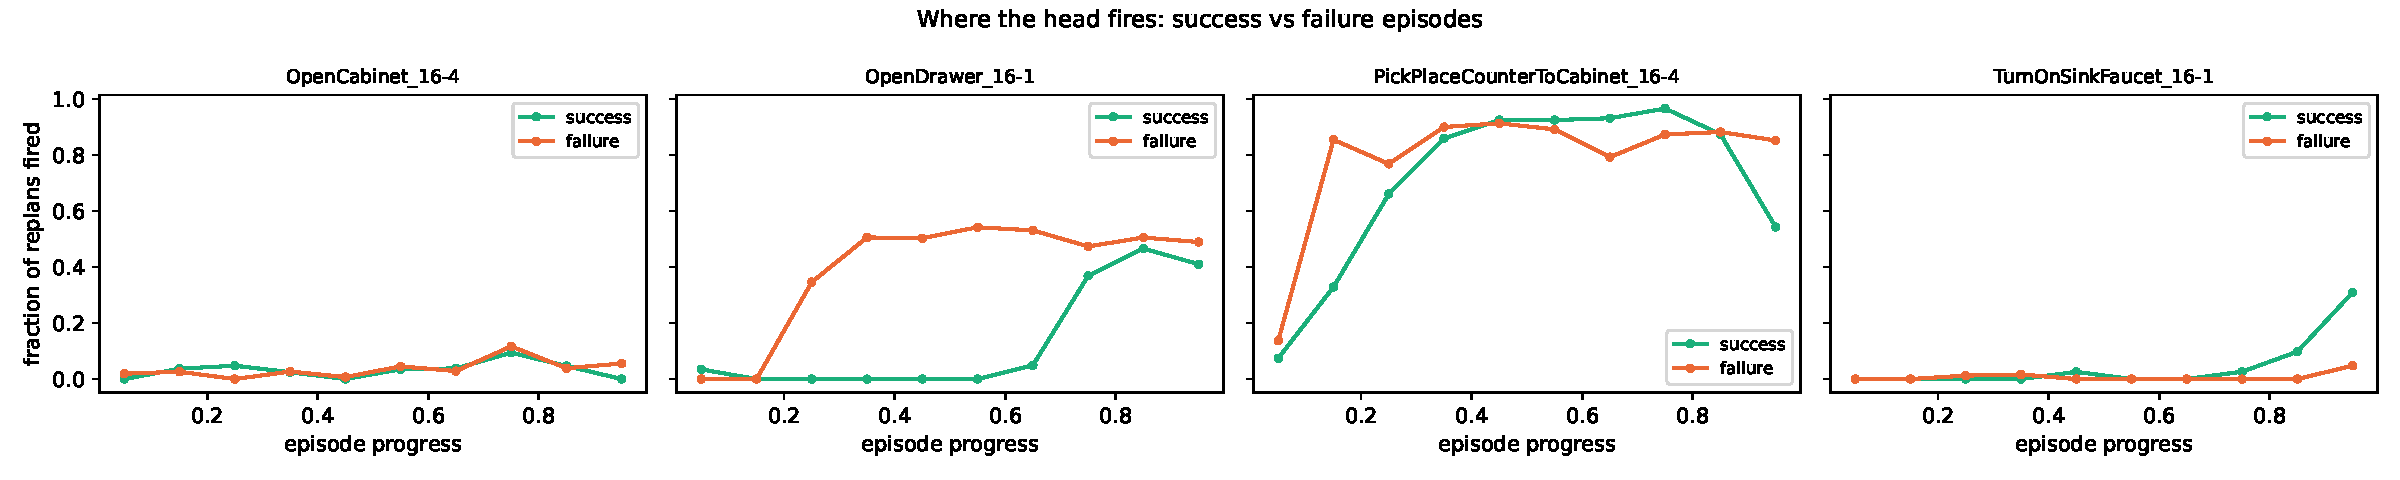
\includegraphics[width=\linewidth]{figs/firing_by_progress.pdf}
\caption{Where the head fires during rollouts, by episode progress, split by
outcome. OpenDrawer failures fire far more than successes; TurnOnSinkFaucet
successes fire slightly more than failures.}
\label{fig:firing}
\end{figure}

%=====================================================================
\section{A stitched long-horizon task with a built-in regime change}
\label{sec:sequence}

The firing-rate bound says switching should show its value on tasks where a
large unstable fraction sits inside a stable frame. We construct one: a
single episode of OpenCabinet followed by PickPlaceCounterToCabinet. The
cabinet doors are forced closed after reset, the policy is first instructed
to open the cabinet (success uses the atomic door predicate), and on success
the instruction switches to the environment's own pick and place command.
The horizon is the sum of the two atomic horizons (1800 steps). Switching
uses the stage-matched heads, the OpenCabinet head during stage 1 and the
PickPlace head during stage 2, each at its own training threshold.

\begin{table}[h]
\centering
\small
\begin{tabular}{lccc}
\toprule
Config & success & stage 1 done & episodes \\
\midrule
fixed 16 & .38 & .66 & 50 \\
fixed 8  & \textbf{.44} & .68 & 50 \\
fixed 4  & .22 & .48 & 50 \\
fixed 1  & .10 & .62 & 50 \\
switched (16,4) & .38 & .68 & 50 \\
switched (16,1) & .38 & .72 & 50 \\
switched (8,4)  & .40 & \textbf{.76} & 50 \\
switched (8,1)  & .26 & .60 & 50 \\
\bottomrule
\end{tabular}
\caption{The stitched task, final numbers at 50 episodes per cell.}
\label{tab:sequence}
\end{table}

The final numbers carry a lesson about sample size before they carry a
lesson about switching. At the halfway mark the switched (16,1) cell led at
.75 over 12 episodes; at 50 episodes it settles to .38. The completed grid
shows the best fixed configuration (k of 8 at .44) matching or beating every
switched cell at the learned threshold, with the best switched cell at .40.
Two systematic effects survive. Fixed 1 confirms the closed-loop failure
mode at long horizon: it opens the cabinet in 62 percent of episodes and
almost never completes the carry within the horizon. And the stage
breakdown still favors switching for reaching stage 2: switched (8,4) gets
there in 76 percent of episodes, the best of any configuration, but gives
the advantage back during the pick and place stage. The signal identifies
the regime change correctly; the chunk-shortening response at the
demo-calibrated threshold does not convert it into completed episodes,
which points at the threshold recalibration discussed above.

%=====================================================================
\section{What happens next}

The remaining steps on this platform are: finish the in-progress stitched
task cells and refresh Table~\ref{tab:sequence}, collect the oracle
switching cells (measured $\lambda$ at each replan, the ceiling for any
predictor) and the PickPlace contact-oracle cell, and fold these numbers
into the cross-platform comparison alongside the MimicGen and LIBERO
results. The $\sigma_u$ sensitivity check is already complete: relabeling at
$\sigma_u = 0.30$ leaves rankings essentially unchanged (Spearman 0.834,
95.4\% flag agreement), so the labels behind the predictor heads stand.

\end{document}
